
\section{Neutron Fluxes Discussion}
\label{sec_fit}

The cross section, measured with beam experiments, represents the sensitivity of a device to thermal or high energy neutrons. However, to have an understanding of the actual error rate, one needs to consider the background radiation fluxes of high energy and thermal neutrons where the device will be located. Error rates are then calculated by multiplying the measured cross sections by the neutron fluxes. We report and discuss FIT rates in~\cite{jsc2020}.

The flux for high energy neutrons in the atmosphere can be precisely estimated considering the altitude, longitude, latitude, and solar activity. However, the environment and the materials that surround a device significantly impact neutron flux and energy.  For instance, the rain droplets of thunderstorms act as moderators slowing high energy neutrons into thermal ones. The thermal neutron flux, as measured in~\cite{ziegler2003}, can be $2\times$ higher during a thunderstorm than on a sunny day. Liquid cooling systems can also have the side effect of significantly increasing the proportion of thermal neutrons that hit a device.

For autonomous vehicles, it is even harder to estimate the thermal neutron flux since the environment can drastically change. For instance, the road material, weather condition, and how much fuel the vehicle has in the tank may impact the neutron flux. Besides, as humans are composed primarily of water (an excellent neutron moderator), the number of passengers will change the thermal neutron flux.

\begin{figure}[tb] 
\centering
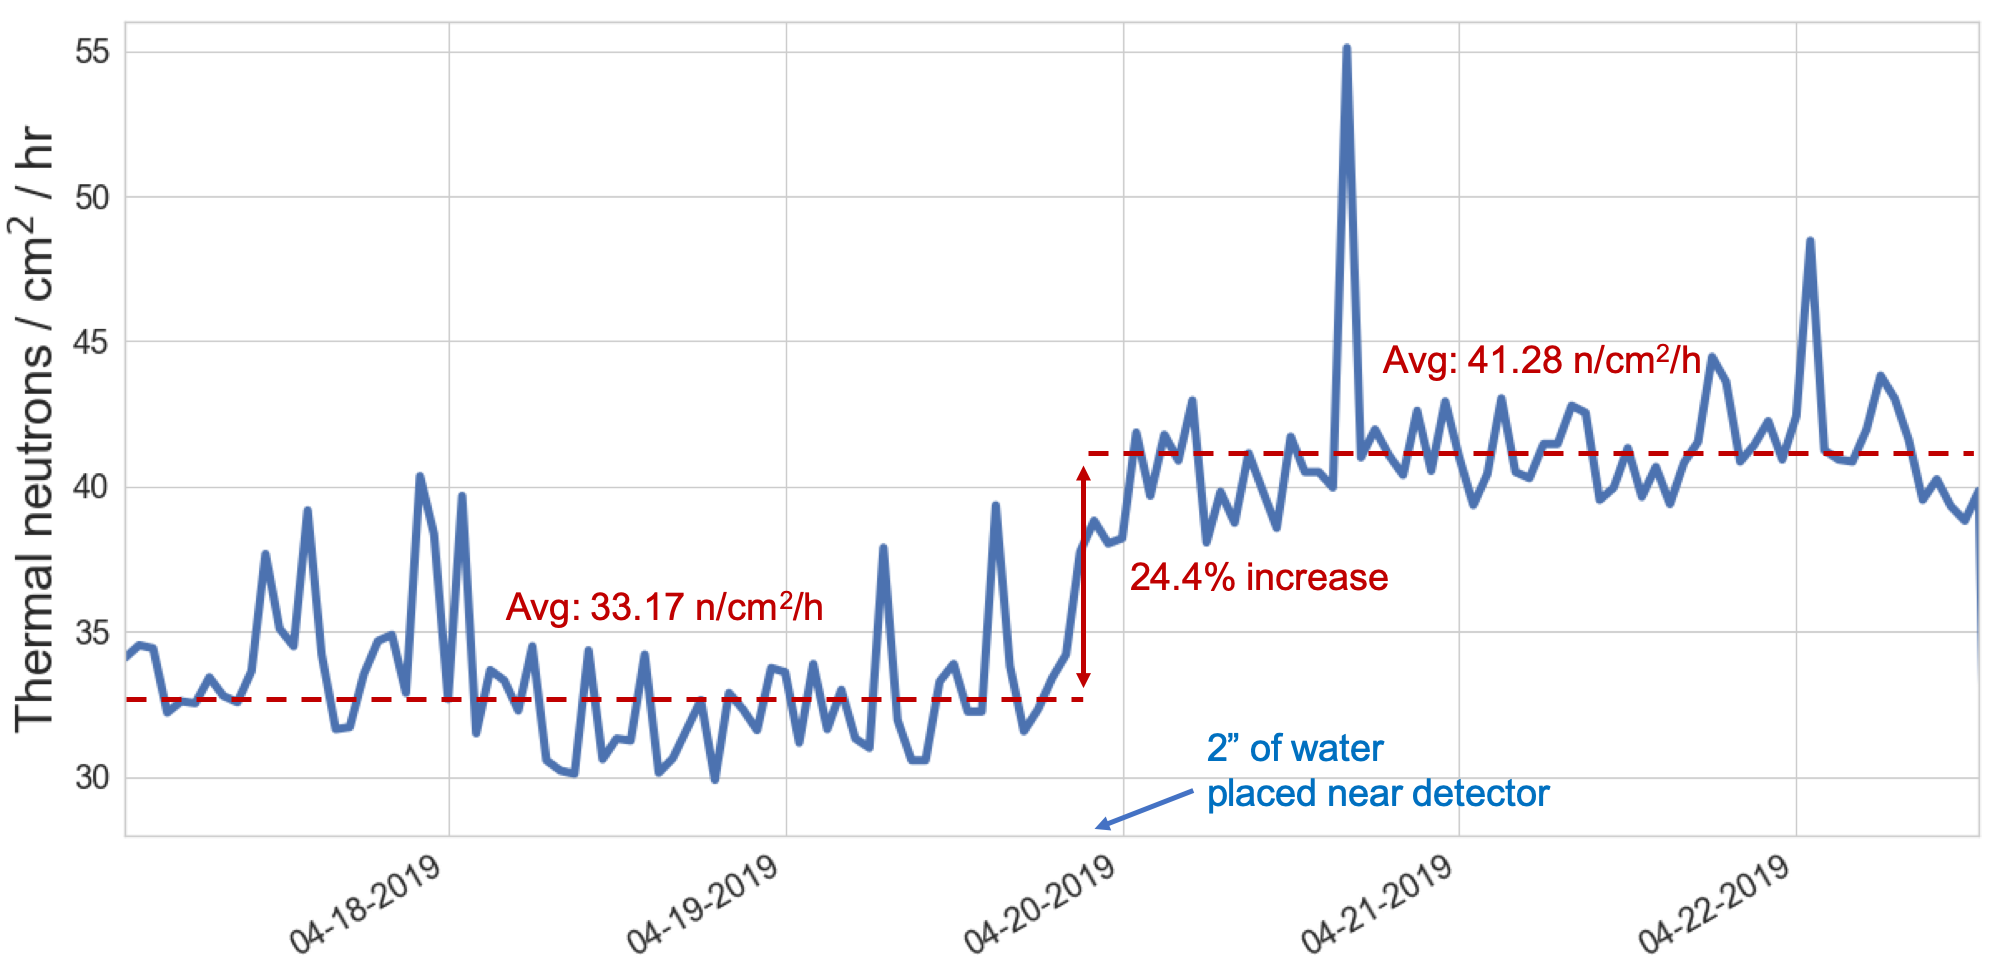
\includegraphics[width=0.82\columnwidth]{./figs/turkeypan_PR}
\caption{Tin-II thermal neutron detector measurements with two inches of water placed over detector on $20^{th}$ April 2019.}
\label{turkeypan}

\end{figure}
\label{sub_flux}

To  empirically measure the impact of materials in the thermal neutron flux in a data center, we placed the Tin-II detector (details in Section~\ref{sub_detector}) in a building similar to the one containing the Trinity supercomputer. We collected data over the course of several days, then placed 2 inches of water in a box over the detector starting on $20^{th}$ April 2019. Figure~\ref{turkeypan} shows that when water is placed over the detector the thermal neutron counts abruptly increase of about 24\%. This increase shows that the presence of water in the cooling system can significantly increase the rates of thermal neutrons in a system, which in turn will increase the rates in the devices sensitive to those neutrons as seen in section~\ref{sec_results}. Considering only the liquid cooling and a concrete floor for a data center, we estimate that the thermal neutron contribution for the total FIT rate of a device can be as high as 40\%~\cite{jsc2020}.

In contrast to high energy neutrons, thermal neutrons flux can be effectively reduced, shielding the device with thin layers of cadmium or some inches of Boron plastic. However, cadmium is highly toxic and should not be heated and, then, it cannot be placed in the proximity of an HPC device or a cooling system. Boron plastic also thermally isolates the device, which makes it impractical to be used as a shield between the cooling system (one of the most efficient sources of thermal neutrons) and the device.


%The cross sections reported and discussed in Section~\ref{sec_results}, represent the device's sensitivity to thermal or high energy neutrons. To have an understanding of the impact of thermal and high energy neutrons in the device error rate, we need to consider also the natural background radiation fluxes of each. FIT rates can then be calculated by multiplying the experimentally measured cross sections by the neutron fluxes. We only show in percentages the contribution of thermal and high energy neutrons to the device's FIT rates to avoid the leakage of business sensitive data. This information allows us to evaluate how much thermal neutrons increases the FIT of each device. This also tells us how much the FIT rate of each device is underestimated if thermal neutrons are not considered.
%
%
%
%\begin{figure*}[!tb]
%    \centering
%    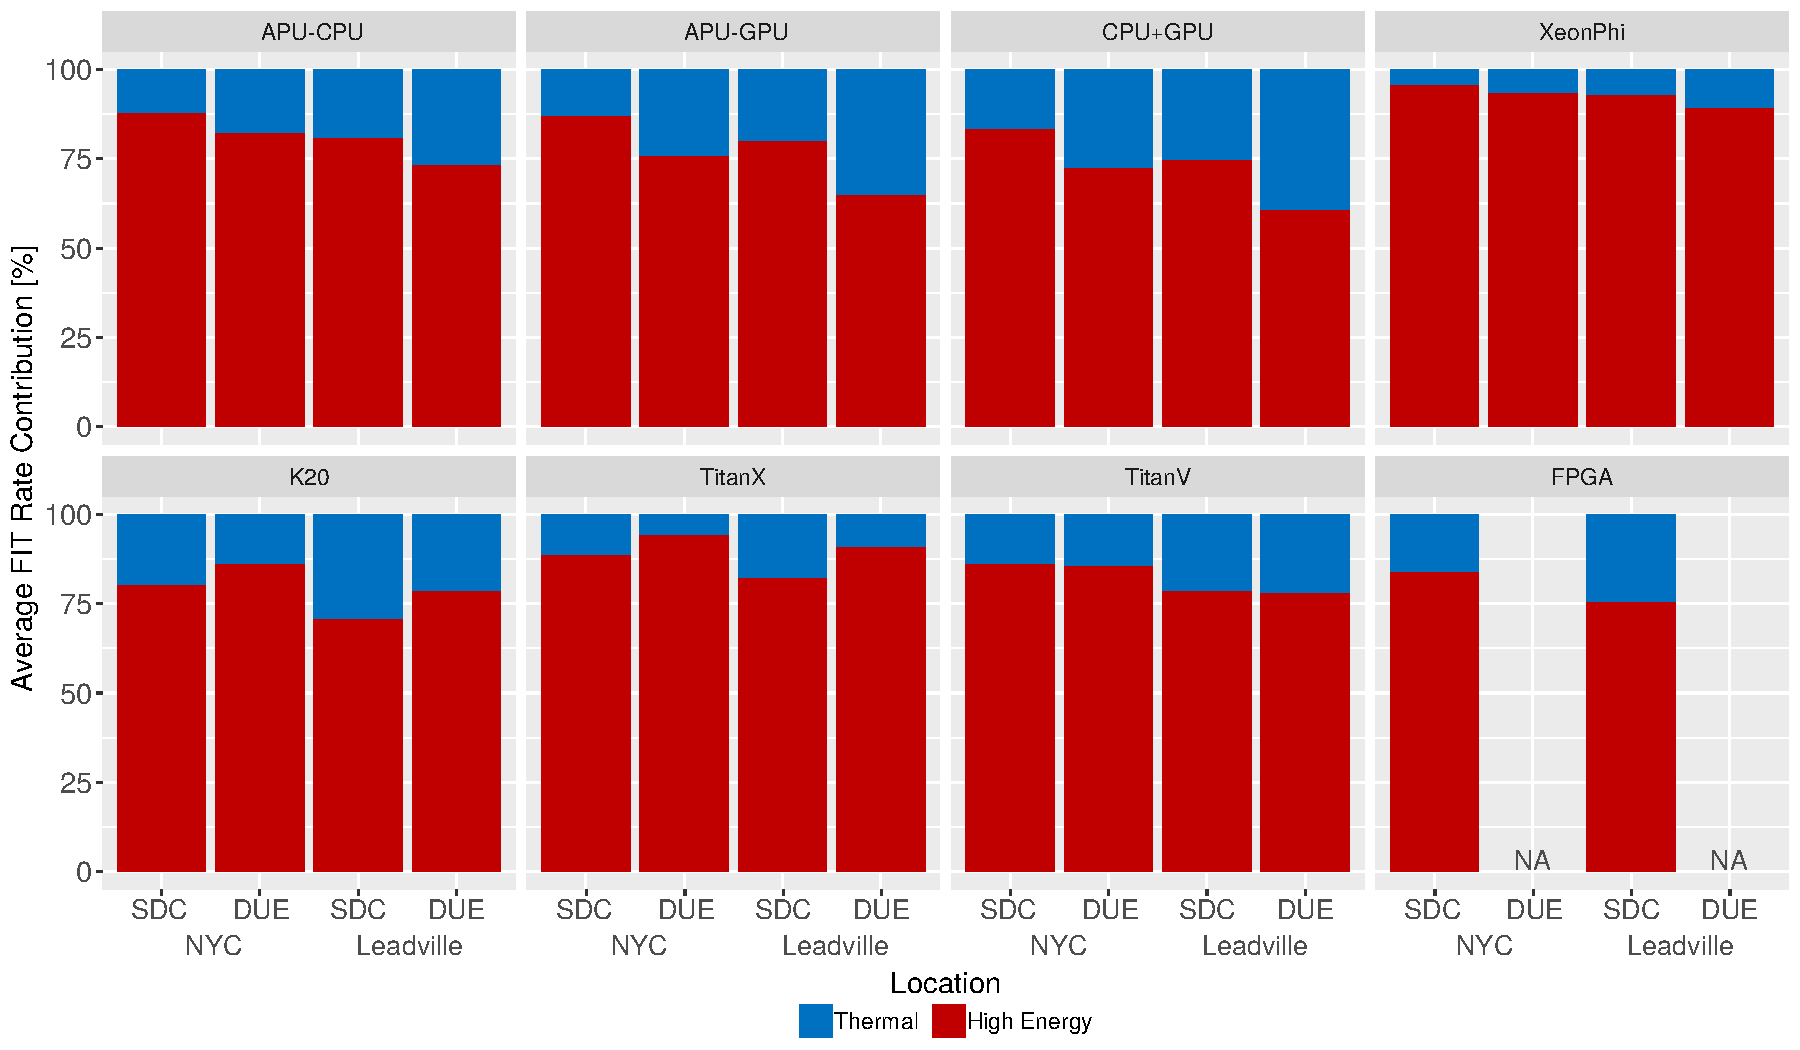
\includegraphics[width=0.85\textwidth]{figs/FIT-rates-all-devices.pdf}
%    \caption{Percentage of total FIT rate due to high energy and thermal neutrons. All tested parts except Xeon Phi show significant errors due to $^{10}B$ levels.}
%    \label{fig_fitpercents}
%\end{figure*}
%
%\label{sub_flux}
%
%The flux for high energy (fast) neutrons in the atmosphere can be precisely estimated considering the
%altitude, longitude, latitude, and solar activity. However, the environment and the materials that surround a device significantly impact neutron flux and energy. 
%For instance, during thunderstorms the rain droplets act as moderators slowing high
%energy neutrons into lower energy ones. The thermal neutron flux, as measured
%in~\cite{ziegler2003}, can be as much as $2\times$ higher during a rain storm than on a sunny day. Thermal neutron rates may be as much as 20\% higher over a large slab of concrete such as in a parking lot or the concrete floor of a machine room. 
%Water cooling systems can also have the side effect of significantly 
%increasing the proportion of thermal neutrons that strike a device.
%
%In order to  empirically measure the impact of materials in the thermal neutron flux in a data center, we placed the Tin-II detector (details in Section~\ref{sub_detector}) in a building similar to the one containing the Trinity supercomputer. We collected data over the course of several days, then placed 2 inches of water in a box over the detector starting on $20^{th}$ April 2019. Figure~\ref{turkeypan} shows that when water is placed over the detector the thermal neutron counts abruptly increase of about 24\%. This increase shows that the presence of water in the cooling system can significantly increase the rates of thermal neutrons in a system, which in turn will increase the rates in the devices sensitive to those neutrons as seen in section~\ref{sec_results}. 
%
%
%These same considerations exist when trying to understand the thermal neutron component of faults in autonomous vehicles. The road material, concrete or asphalt, the vehicle is driving on makes a difference, as does the weather, and the type and volume of fuel the vehicle uses. In addition, the number of passengers will change the thermal neutron flux, as humans are primarily composed of water  which makes us excellent neutron moderators. 
%
%\subsection{High Energy vs Thermal Neutrons FIT}
%
%
%Figure~\ref{fig_fitpercents} shows the percentage of the total FIT rates due to high energy and thermal neutrons. These calculations use measured values of neutrons at sea level (NYC) and in Leadville, CO (10,151 ft in altitude). The thermal rates used have been adjusted to compensate for back scattered neutrons from a concrete slab and water cooling as measured by Tin-II detector, an overall increase of 44\% in the thermal flux. Note that on a rainy day the thermal flux may be as much as doubled over the rates used in this graph and the corresponding FIT rate on those days will increase in a corresponding way~\cite{ziegler2003}.
%
%Xeon Phi processors, 
% as stated in Section~\ref{sec_results}, have a low sensitivity to thermals, which is a symptom of the use of either depleted boron or a reduction in boron usage. 
% Thus, the thermals FIT rate seen in figure~\ref{fig_fitpercents} is a relatively small percentage of the overall FIT rate (from 4.2\% at NYC SDC up to 10.6\% for Leadville DUE).
%The other tested devices, especially the K20 and CPU+GPU devices, have thermal FIT rates comparable to the FIT rates from high energy neutrons. At Leadville, K20 has 29\% of the SDC FIT rate caused by thermal neutrons while APU CPU+GPU has 39\% of DUEs caused by thermal neutrons.
%
%\subsection{Discussion}
%
%
%Figure~\ref{fig_fitpercents} shows that if thermal neutrons contribution to the device error rate is not considered both the DUE and SDC FIT rates could be significantly underestimated, posing unconsidered risks to a safety critical application or reducing the HPC server productivity unexpectedly. 
%Of particular interest in Figure~\ref{fig_fitpercents} is the relatively high percentage of
%faults that result in Silent Data Corruption (SDC) on several of the tested devices. In general, HPC systems are designed and engineered to maintain SDC rates low and manageable, where corrupted calculations are rare and often noticeable to users. However, anything that increases the SDC rate is always concerning. In safety critical applications, SDCs should be strictly avoided as they could put the system in unexpected states, and they could potentially lead to unpredictable actions.
%
%The elevated DUE rates are also of concern as they result in a system crash and loss of some portion of a calculation's run time. 
%It is worth noting that even with thin layers of shielding, embedded devices in vehicles can suffer from a much higher thermal flux than the one considered in Figure~\ref{fig_fitpercents} due to moderation and reflection from the surrounding materials~\cite{leo2012techniques}.

%%%%Our analysis shows that thermal neutrons are a threat for the reliability of supercomputers and safety critical applications that rely on COTS HPC devices. While the benefits in terms of cost, performances, and efficiency of COTS devices are not in question, their utilization in applications for which reliability is a concern must be coupled with a careful reliability evaluation that considers the impact of thermal neutrons. As the amount of $^{10}B$ in the manufacturing process is not publicly available, radiation experiments are one of the few ways to evaluate the sensitivity of a COTS device to thermal neutrons. %Moreover, as the thermal neutron flux strongly depends on environmental conditions, the device error rate varies significantly when conditions change. Therefore it is critical to consider the realistic conditions in which the device will operate and estimate the correspondent thermal neutrons flux. These conditions have a direct impact on HPC applications. For instance, when supercomputer time is allocated, the checkpoint frequency may need to  consider weather conditions.
%%%%Dissimilarly to high-energy neutrons, thermal neutrons flux can be effectively reduced shielding the device with thin layers of cadmium or some inches of boron plastic. Unfortunately, cadmium is highly toxic and should not be heated, so it should not be placed in the proximity of an HPC device or of a cooling system, and boron plastic also thermally isolate the device, so it is impractical to be used as a shield between the cooling system (one of the most efficient sources of thermal neutrons) and the device. 

